% !TEX encoding = UTF-8
% !TEX TS-program = pdflatex
% !TEX root = ../tesi.tex

%**************************************************************
\chapter{Algoritmi di Machine Learning}
\label{cap:ML}
%**************************************************************
\intro{Questo capitolo illustrerà i metodi di \emph{machine Learning} che sono stati utilizzati per la predizione degli esiti delle partite di calcio della Seria A italiana della stagione 2021/2022. Purtroppo, non è stato possibile applicare metodi di \emph{machine learning} che corrispondessero al modello \emph{Bradley-Terry} perché, nonostante esistano metodi in \emph{machine learning} che forniscono modelli basati sul modello \emph{Bradley-Terry}, essi non sono in grado di gestire l'esito del pareggio ma solo un esito binario. Ne consegue che tali metodi non sono adatti per contesti come il calcio ma ad altri tipi di sport dove il pareggio non è previsto come il \emph{baseball}. I metodi di \emph{machine learning} considerati sono: il K-Nearest-Neighbors (K-NN), la Support Vector Machine (SVM), gli alberi di decisione per la classificazione, la Random Forest e infine l'AdaBoost.
}
\section{Componenti essenziali}
In questa sezione vengono definite alcune misure e tecniche che sono necessarie l'applicazione dei metodi di \emph{machine Learning} applicati.
\subsection{Distanza di Minkowski}
La distanza di Minkowski (vedi \textit{\cite{minkdist}}) è una misura utilizzata per la valutazione della distanza ovvero, nel nostro contesto, della somiglianza tra due punti in uno spazio di \textit{n}-dimensioni. La distanza di Minkowski di ordine \emph{d} tra due punti A = (a$_1$,...a$_n$) e B = (b$_1$,...b$_n$) è definita come
\begin{center}
	$Dist(A,B) =  \left(\sum_{i = 1}^{n}|a_i-b_i|^d\right)^{1/d} $.
\end{center}

Si sottolinea che per d = 1, la distanza utilizzata è la distanza di Manhattan (vedi\textit{\cite{manhattan}}), ovvero la distanza tra due punti è la somma del valore assoluto delle differenze delle loro coordinate. Quando d = 2, è applicata la distanza Euclidea (vedi \textit{\cite{euclidea}}), secondo la quale la distanza tra due punti è la lunghezza del segmento con agli estremi i due punti d'interesse.
Tale misura sarà utilizzata nel metodo K-Nearest-Neighbors (K-NN).
\subsection{Funzione kernel}
Nel contesto dell'apprendimento automatico, la \textit{\cite{kernel}} permette di trasformare uno spazio di input non linearmente separabile in un nuovo spazio delle istanze di input detto \emph{feature space} di dimensione superiore rispetto a quello originale e tale da diventare linearmente separabile. Per spazio linearmente separabile si intende un iperpiano in grado di separare correttamente i dati in due gruppi distinti. Perciò, aumentando la dimensionalità dello spazio d'interesse è possibile trovare la dimensione opportuna che permetta di separare linearmente i dati. Tale applicazione è chiamata \emph{kernel trick}. Una funzione kernel è una funzione \emph{K} che per ogni \emph{x}, \emph{y} $\in \chi$, dove $\chi$ è lo spazio di input di dimensione \emph{n}, vale 
\begin{center}
	$K(x,y) =  \langle\psi(x),\psi(y)\rangle $,
\end{center}
con $\psi$ funzione che mappa i punti di uno spazio di dimensione \emph{n} in uno spazio di dimensione \emph{m} con \emph{m>n}, e $\langle . \rangle$ prodotto scalare.\\
Nelle nostre predizioni saranno usati i seguenti kernel:
\begin{itemize}
	\item linear kernel, è la funzione precedentemente definita;
	\item polynomial kernel, $K(x,y) =  \left(1 + \sum_{i = 1}^{p}x_iy_i\right)^{d} $, dove \emph{p} è il numero di istanze di input presenti in $\chi$ e \emph{d} la dimensione del spazio (l'ordine);
	\item Gaussian Radial Basis kernel (RBF), $K(x,y) = exp(-\gamma||x-y||^2) $, con $\gamma=\frac{1}{2\sigma^2}$ e $\sigma$ paramento libero. 
\end{itemize}

Nella Figura \ref{fig:kernel} è mostrato un esempio di applicazione della funzione kernel.\\

\begin{figure}[h]
	\begin{center}
		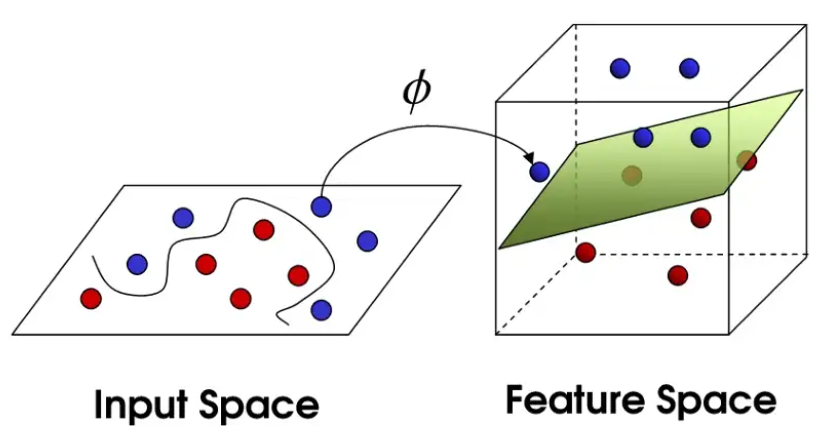
\includegraphics[scale=0.50]{kernel.png}
		\caption{Esempio grafico della funzione kernel $\gamma$ mappa i punti di uno spazio d'input in uno feature space di dimensione maggiore e linearmente separabile.
		} 
		Source: \url{https://towardsdatascience.com/the-kernel-trick-c98cdbcaeb3f}\label{fig:kernel}
	\end{center}
\end{figure}

La funzione kernel sarà utilizza nella Support Vector Machine (SVM).

\subsection{Bootstrap}
In statistica e nell'apprendimento automatico, per Bootstrap (vedi \textit{\cite{bootstrap}}) si intende una tecnica di ricampionamento per la generazione di un insieme di campioni di \emph{m} osservazioni contenute in un dataset di dimensione \emph{n}. Ogni estrazione è casuale e con reinserimento, cioè un’osservazione può essere presente in più campioni. Tale tecnica è utilizzata per produrre un insieme di campioni che siano il più possibile rappresentativi e indipendenti tra di loro.\\
Nella Figura \ref{fig:bootstrap} viene mostrato un esempio della procedura di Bootstrap

\begin{figure}[h]
	\begin{center}
		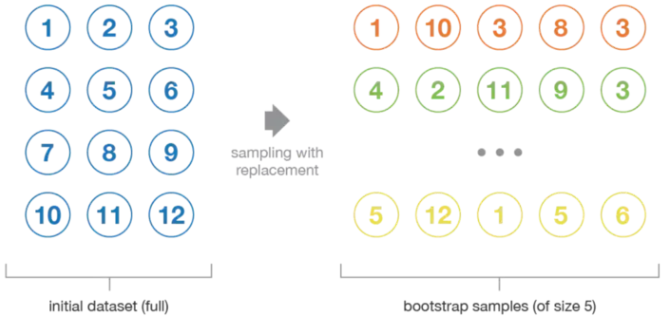
\includegraphics[scale=0.60]{bootstrap1.png}
		\caption{Esempio grafico della procedura di Bootstrap.
		} 
		Source: \url{https://blog.paperspace.com/bagging-ensemble-methods/}\label{fig:bootstrap}
	\end{center}
\end{figure}

\subsection{Bagging}
Il Bagging \autocite{breiman1996bagging} detto anche \emph{Bootstrap Aggregation Approach}, è una tecnica di \emph{ensemble learning} di tipo parallelo che dalla mediazione di più predizioni fatte da un insieme di classificatori deboli ottiene un'unica predizione finale. È di tipo parallelo perché va a sfruttare l'indipendenza dei classificatori. La procedura applicata è la seguente:
\begin{itemize}
	\item creazione di \emph{k} campioni utilizzando la tecnica di Bootstrap,
	\item per ogni campione, allenare un classificatore,
	\item produrre una predizione per ogni classificatore allenato,
	\item ottenere una media delle predizioni per avere una predizione finale.
\end{itemize} 
Una tecnica per ottenere una media è, ad esempio, il \emph{voting} secondo il quale la classe più predetta sarà il risultato dalla predizione finale. Inoltre, si utilizza il Bootstrap per rendere i classificatori indipendenti tra di loro.
Perciò l'obbiettivo del Bagging è quello di creare un classificatore in grado di gestire un'elevata varianza dei dati in modo efficiente grazie al parallelismo.\\
Nella Figura \ref{fig:bagging} viene illustrato graficamente la procedura di Bagging.

\begin{figure}[h]
	\begin{center}
		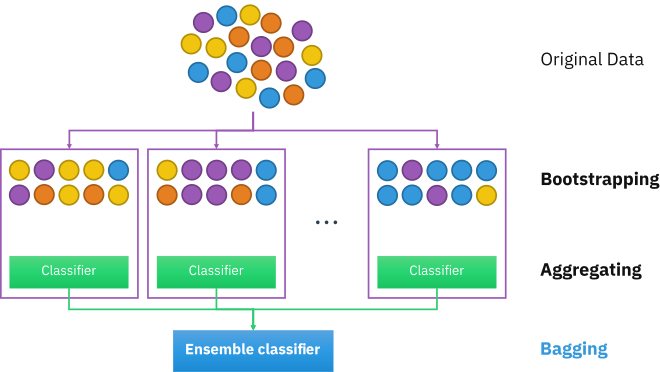
\includegraphics[scale=0.50]{Ensemble_Bagging.png}
		\caption{Esempio grafico della procedura di Bagging.
		} 
		Source: \url{https://www.analyticsvidhya.com/blog/2020/02/what-is-bootstrap-sampling-in-statistics-and-machine-learning/}\label{fig:bagging}
	\end{center}
\end{figure}

\subsection{Boosting}
Il Boosting \autocite{freund1996experiments} è una tecnica di \emph{ensemble learning} di tipo sequenziale che sfrutta la dipendenza tra i classificatori usati. L'algoritmo inizialmente allena un classificatore debole con tutto il \emph{dataset} a disposizione. Successivamente, per raffinare la predizione, vengono allenati in sequenza nuovi classificatori che apprendono da tutto ciò che è stato appreso dal classificatore precedente utilizzando ancora l'intero \emph{dataset}.\\
La procedura completa è la seguente:
\begin{itemize}
	\item viene utilizzato l'intero \emph{dataset} per allenare un classificatore debole;
	\item vengono ripesati gli esempi di \emph{training} dando un peso maggiore a quei esempi classificati erroneamente, viceversa per gli esempi classificati correttamente,
	\item ripetere per \emph{n} volte i passi precedenti con un nuovo classificatore con i pesi aggiornati;
	\item combinare tutte le ipotesi semplici in un unico classificatore accurato per ottenerne il risultato finale.
\end{itemize}
Con l'aggiornamento dei pesi si presuppone che i classificatori successivi non andranno a commettere gli stessi errori dei classificatori precedenti.\\
L'obbiettivo del Boosting è concentrare i propri sforzi nel creare un classificatore adatto a gestire un'elevata distorsione, anziché un'elevata varianza dei dati. Infatti, partendo da un classificatore debole e migliorandolo in modo sequenziale, si consente ai classificatori successivi di imparare dagli errori precedentemente commessi, riducendo la distorsione dei dati. Inoltre, il Boosting ha una buona resistenza agli effetti dell'\emph{overfitting}.
Purtroppo, il Boosting risulta molto sensibile ai valori anomali. Inoltre, dato che le operazioni di addestramento di ogni classificatore avvengo in modo sequenziale, non sarà possibile utilizzare il parallelismo per risparmiare tempo di calcolo.\\
Nella Figura \ref{fig:boosting} viene illustrata la procedura di Boosting.

\begin{figure}[h]
	\begin{center}
		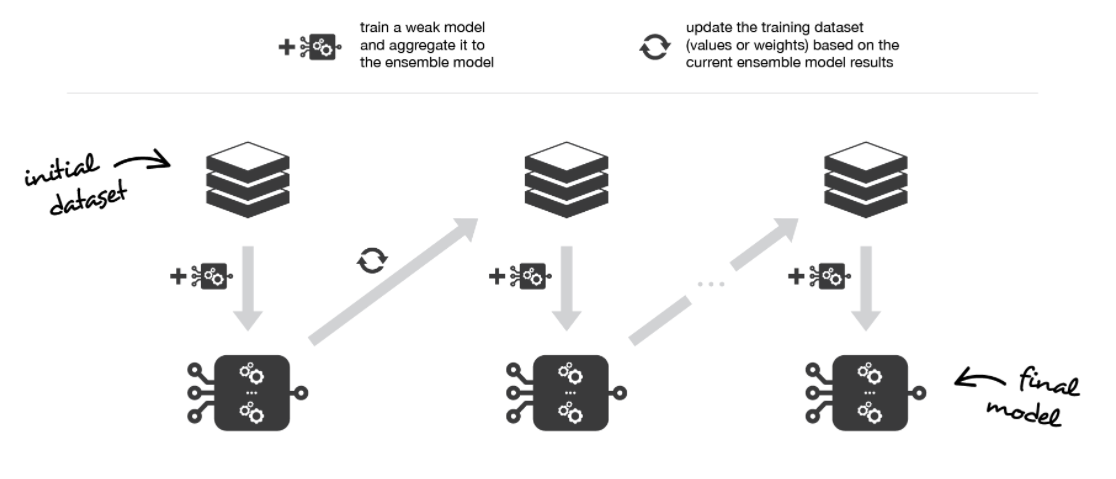
\includegraphics[scale=0.55]{boosting.png}
		\caption{Esempio grafico della procedura di Boosting.
		} 
		Source: \url{https://www.section.io/engineering-education/boosting-algorithms-python/}\label{fig:boosting}
	\end{center}
\end{figure}

\section{K-Nearest-Neighbors}
Il K-Nearest-Neighbors (K-NN) \autocite{dasarathy1991nearest} è un algoritmo di apprendimento automatico di tipo supervisionato che permette la classificazione delle istanze ricevute in input. Inoltre, ne esiste una versione per problemi di regressione. Il K-NN assume che tutte le istanze corrispondano a punti in uno spazio di dimensionalità \emph{n} e utilizza la prossimità tra i vari punti per classificarli, ossia classifica l'istanza con la classe maggiormente presente tra i punti attorno all'istanza stessa, detti punti vicini. Fondamentale, perciò, è l'utilizzo di una qualche tecnica di misurazione della distanza per individuare chi sono i vicini dell'istanza da classificare, ossia la distanza tra il nostro punto d'interesse rispetto a tutti gli altri punti. La misura di distanza maggiormente utilizzata è la distanza di Minkowski definita nella sezione precedente. Misurati tutti i punti, occorre stabilire poi quanti dei punti presenti devono essere considerati vicini. A questo scopo, va fissato il valore di \emph{k}, iperparametro dell'algoritmo che stabilisce di considerare solo i \emph{k} punti più vicini all'istanza da classificare. Per esempio, se \emph{k = 3}, si considerano i tre punti più vicini e si classifica l'istanza con la classe più frequente tra i tre punti considerati. È importante scegliere il corretto valore di \emph{k}, dato il rischio di \emph{overfitting}, nel caso si considerino punti troppi vicini, o \emph{underfitting}, nel caso si considerino pochi punti vicini. Infatti, con valori più bassi di \emph{k} può verificarsi un'elevata varianza e una distorsione bassa, mentre con valori più grandi di \emph{k} può verificarsi un'elevata distorsione e una varianza bassa delle predizioni. Una buona soluzione per la scelta dell'iperparametro \emph{k}, così come dell'ordine \emph{p} della distanza da utilizzare, è la Cross Validation.\\
Nella Figura \ref{fig:knn} è mostrato un esempio di applicazione dell'algoritmo K-NN.\\
\begin{figure}[h]
	\begin{center}
		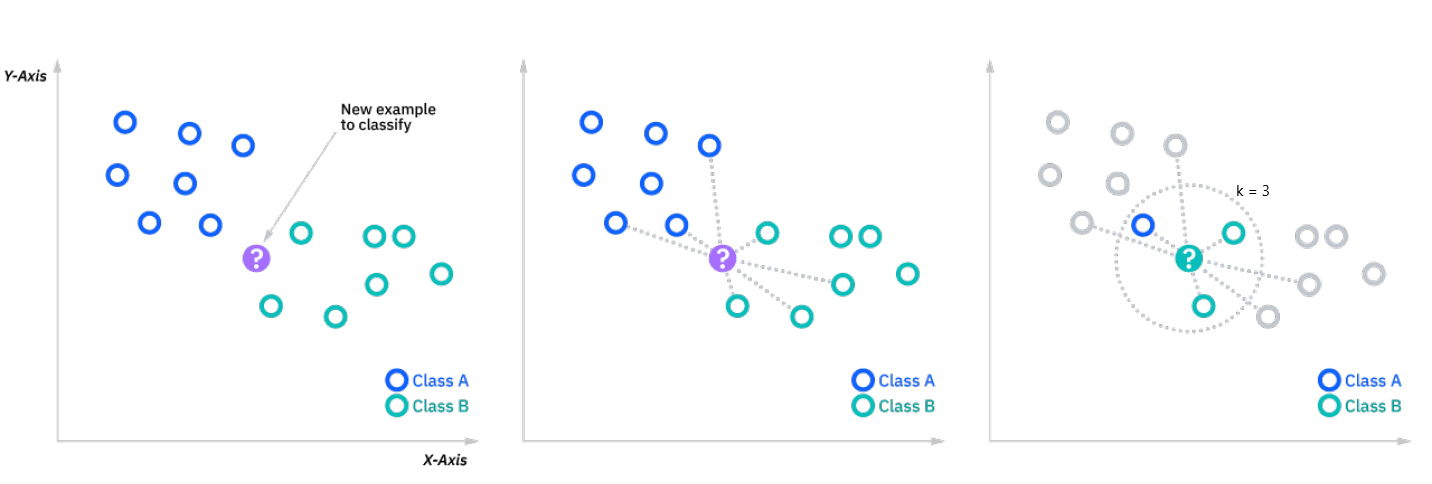
\includegraphics[scale=0.40]{knn.png}
		\caption{Esempio grafico dell'algoritmo K-Nearest-Neighbors.
			L'istanza da classificare è indicata con il punto interrogativo (?).
			Il primo passo dell'algoritmo è quello di calcolare tutte le distanze. Dopo di che, considera solo i \emph{k = 3} punti più vicini all'istanza (?). Infine l'algoritmo classifica con la classe B l'istanza (?).
		} 
		Source: \url{https://www.ibm.com/topics/knn#:~:text=The%20k%2Dnearest%20neighbors%20algorithm%2C%20also%20known%20as%20KNN%20or,of%20an%20individual%20data%20point.}\label{fig:knn}
	\end{center}
\end{figure}

Il K-NN è un algoritmo di classificazione non parametrico, ovvero non fa alcuna assunzione sulla forma della distribuzione dei dati. Inoltre, dato che è un algoritmo di apprendimento supervisionato, le istanze d'input sono nella forma $(x, f(x))$. Nella fase di 
addestramento si limita soltanto a memorizzare i dati di \emph{training}, dato che li utilizza direttamente per fare predizione. Purtroppo, però, la fase di predizione può essere lenta, poiché è necessario calcolare la distanza di ogni osservazione dall'istanza da classificare, con un costo computazionale crescente se vi sono molti dati.

\section{Support Vector Machine}
La Support Vector Machine (SVM) \autocite{GHOLAMI2017515} è un algoritmo di apprendimento automatico di tipo supervisionato applicabile in contesti di classificazione. La SVM considera le istanze del \emph{dataset} come punti in uno spazio di dimensionalità \emph{n} è il suo obbiettivo è quello di costruire l'iperpiano ottimo che separi in due classi le osservazioni. L'iperpiano ottimo viene scelto in modo tale da ottenere il maggior margine possibile tra le due classi, ovvero il maggior spazio possibile tra le osservazioni di ciascuna classe e l'iperpiano. Il nome di quest'algoritmo deriva dall'utilizzo dei vettori detti vettori di supporto. Questi vettori sono le istanze che si trovano più vicino all'iperpiano ovvero quelli più difficili da classificare e quindi danno un grosso contributo alla costruzione dell'iperpiano rispetto alle altre osservazioni. Perciò per massimizzare la distanza tra l'iperpiano e i punti di entrambe le classi, occorre risolvere il seguente problema di ottimizzazione vincolata, 
\begin{align}
	\text{min} & \frac{1}{2} \|\mathbf{w}\|^2 + C \, \sum_{i=1}^{n} (\xi_i) \label{for:6.3}
\end{align}
\begin{align*} 
	\begin{cases}
		y_i(\mathbf{w \cdot x}_i + b) \geq  1 - \xi_i \\
		\xi_i \geq 0, i=\{1,...,n\}
	\end{cases} \, .
\end{align*}
Nel problema \ref{for:6.3} $\|\mathbf{w}\|$ è il vettore direzione e l'iperparametro \emph{C} è un parametro di regolarizzazione, il quale permette di gestire il \emph{trade-off} tra massimizzazione del margine e penalizzazione, consentendo di controllare la complessità del modello e, quindi, di prevenire l'\emph{overfitting}. Il parametro $\xi_i$ è l'errore commesso. La quantità $\mathbf{w \cdot x}_i + b$ è la distanza algebrica tra l'iperpiano scelto e il punto più vicino.\\
Nella Figura \ref{fig:svm} è mostrato un esempio di applicazione dell'algoritmo SVM.
\begin{figure}[h]
	\begin{center}
		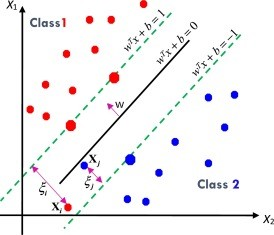
\includegraphics[scale=0.80]{svm.jpg}
		\caption{Esempio grafico dell'algoritmo Support Vector Machine. I punti sulle linee trattegiate indicano i vettori di supporto, mentre la retta al centro indica l'iperpiano ottimo di separazione.
		} 
		Source: \url{https://www.sciencedirect.com/science/article/pii/B9780128113189000272}\label{fig:svm}
	\end{center}
\end{figure}
L'algoritmo SVM è grado di gestire anche spazi d'input non linearmente separabili, grazie all'utilizzo della funzione kernel definita nella sezione precedente. Tramite la Cross Validation si sceglierà il valore più opportuno per l'iperparametro \emph{C} e il tipo di kernel da applicare.

\section{Decision Tree}
Un Decision Tree \autocite{charbuty2021classification} è un algoritmo di apprendimento automatico di tipo supervisionato e non parametrico che utilizza una struttura ad albero per produrre le proprie predizioni. Tale albero contiene un insieme di nodi in cui, per ogni nodo, vi è un test su un attributo dell'osservazione da classificare. Perciò, ad ogni nodo, ci sarà una scelta da compiere in base al valore contenuto dell'attributo, che porterà verso un nuovo ramo oppure a una foglia. Le foglie contengono i risultati della classificazione. L'approccio utilizzato per la costruzione dell'albero di decisione è di tipo \emph{greedy}, cioè ogni scelta effettuata su un nodo è l'opzione più conveniente in quel momento. L'albero viene costruito in modalità \emph{top-down} secondo i seguenti passi:
\begin{itemize}
	\item viene creata la radice \emph{T} dell'albero;
	\item se le osservazioni dell'insieme \emph{D} sono tutte della stessa classe \emph{k}; allora viene ritornata la radice \emph{T} classificata con la classe \emph{k};
	\item se le osservazioni non hanno attributi che li descrivono, allora viene ritornata la radice \emph{T} classificata con la classe di maggior presenza tra le osservazioni;
	\item viene scelto un attributo \emph{a}, in base a una specifica regola;
	\item viene partizionato \emph{D} a seconda dei \emph{m} valori che può assumere l'attributo \emph{a};
	\item vengono creati ricorsivamente i sottoalberi dall'albero con radice \emph{T} senza l'attributo \emph{a} ripetendo i passi appena descritti.
\end{itemize} 
Un iperparametro di quest'algoritmo è la regola per la decisione di quale attributo testare in un nodo. Nel presente lavoro saranno considerate le seguenti regole:
\begin{itemize}
	\item Cross Entropy: È la misura del grado di impurità di un insieme di osservazioni. Sia \emph{m} il numero di classi e $D_k$ il sottoinsieme di $D$ di osservazioni di classe \emph{k}, allora l'entropia vale
	\begin{align*}
		I_E =	- \sum_{k=1}^{m} p_k log(p_k),
	\end{align*} 
	dove $p_k$ è la probabilità di estrarre un'osservazione di classe \emph{k}, ovvero vale $\frac{|D_k|}{|D|}$.
	\item Gini Index: È la misura di quanto spesso un'osservazione estratta casualmente dall'insieme delle osservazioni è classificata in modo errato basandosi solo sulla distribuzione delle classi. Sia \emph{m} il numero di classi e $D_k$ il sottoinsieme di $D$ di osservazioni di classe \emph{k}, allora l'indice di Gini vale
	\begin{align*}
		I_G = 1 - \sum_{k=1}^{m} p_{k}^2,
	\end{align*} 
	dove $p_k$ è la probabilità di estrarre un'osservazione di classe \emph{k}, ovvero vale $\frac{|D_k|}{|D|}$.
\end{itemize}
Per scegliere l'attributo da valutare ad ogni nodo, si fa riferimento all'\emph{information gain}
\begin{align*}
	G(D,a) = I_x - \sum_{v\in V(a)} \frac{|D_a = v|}{D}I_x(D_a=v),
\end{align*} 
dove $I_x$ è la regola scelta e $D_a=v$ è l'insieme delle istanze con valore \emph{v} nell'attributo \emph{a}.
L'attributo che viene scelto per il test nel nodo è quello con il maggior valore nell'\emph{information gain}.\\
Il Decision Tree è un modello facile da interpretare e utilizzare, tuttavia, può essere suscettibile all'\emph{overfitting}. È opportuno, perciò, attraverso la Cross Validation, scegliere il valore da assegnare all'iperparametro del limite della massima profondità dell'albero per limitarne la complessità.
\section{Random Forest}
Il Random Forest \autocite{ho1995random} è un algoritmo di apprendimento automatico basato sull'utilizzo della tecnica di Bagging applicato ad un insieme di Decision Tree utilizzati per la classificazione. L'obbiettivo dell'algoritmo è ottenere una bassa correlazione tra gli alberi e quindi ridurre la varianza. Per tale motivo viene utilizzato il Bagging per addestrare gli alberi di decisione. Tramite con il Bootstrap viene quindi creata una serie di campioni di esempi di training, in cui ogni campione ha un sottoinsieme di attributi e viene utilizzato per addestrare un'albero di decisione. Una volta che sono stati costruiti gli alberi, viene fatta la predizione per ogni modello e, attraverso un algoritmo di mediazione, ad esempio il \emph{voting}, viene prodotta la predizione finale.\\
La Random Forest è in grado di ridurre l'\emph{overfitting} che può verificarsi con l'utilizzo di un singolo albero di decisione. Tuttavia, richiede una quantità significativa di risorse computazionali per la costruzione dei singoli alberi di decisione e può essere meno interpretabile rispetto a un singolo albero di decisione.\\
Nella Figura \ref{fig:forest} è mostrato un esempio di applicazione dell'algoritmo Random Forest.
\begin{figure}[h]
	\begin{center}
		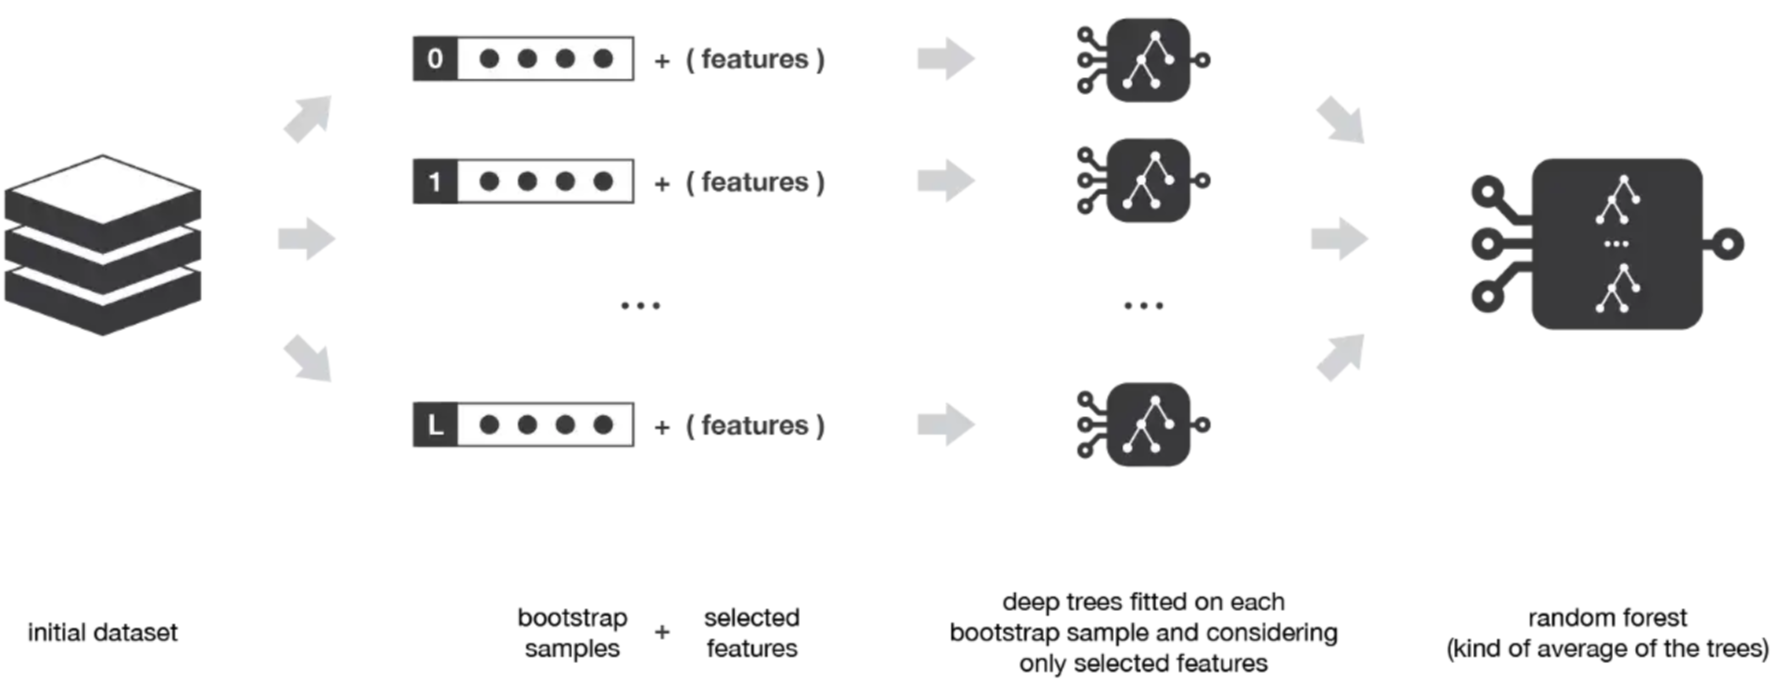
\includegraphics[scale=0.35]{forest.png}
		\caption{Esempio grafico dell'algoritmo Random Forest.
		} 
		Source: \url{https://towardsdatascience.com/ensemble-methods-bagging-boosting-and-stacking-c9214a10a205}\label{fig:forest}
	\end{center}
\end{figure}
Gli iperparametri utilizzati sono gli stessi del Decision Tree con l'aggiunta dell'iperparametro che indica il numero di alberi di decisione scelto tramite Cross Validation.
\section{AdaBoost}
L'algoritmo di AdaBoost (Adaptive Boosting) \autocite{auer1995gambling} è un algoritmo di apprendimento supervisionato che utilizza la tecnica di Boosting per creare un modello di classificazione accurato a partire da un insieme di classificatori deboli. Ad ogni iterazione, i pesi assegnati alle osservazioni vengono modificati dando maggior peso alle istanze che sono state classificate erroneamente per procedere con l'addestramento di un nuovo classificatore debole. L'obbiettivo dei classificatori deboli è quello di massimizzare l'accuratezza del peso, ovvero, minimizzare l'errore $\xi_t$
\begin{align*}
	\xi_t = \sum_{i} D_{t}(i)[h_{t}(x_{i}) \neq y_{i}],
\end{align*} 
dove $D_{t}$ è la distribuzione dei pesi della \emph{t}-esima iterazione. La funzione $h_{t}(x_{i})$ indica il risultato prodotto dal classificatore debole nell'\emph{i}-esima istanza mentre $ y_{i}$ è il target dell'\emph{i}-esima istanza. Perciò la variazione del peso $\alpha_t$ di ogni classificatore viene calcolato tenendo conto dell'errore $\xi_t$,
\begin{align*}
	\alpha_t = \frac{1}{2}log\frac{1-\xi_t}{\xi_t}.
\end{align*} 
Una volta calcolato $\alpha_t$, i pesi vengono modificati dando più peso alle osservazioni classificate in modo errato. Viceversa per le osservazioni classificate correttamente.\\
Nella Figura \ref{fig:ada} è mostrato un esempio di applicazione dell'algoritmo AdaBoost.
\begin{figure}[h]
	\begin{center}
		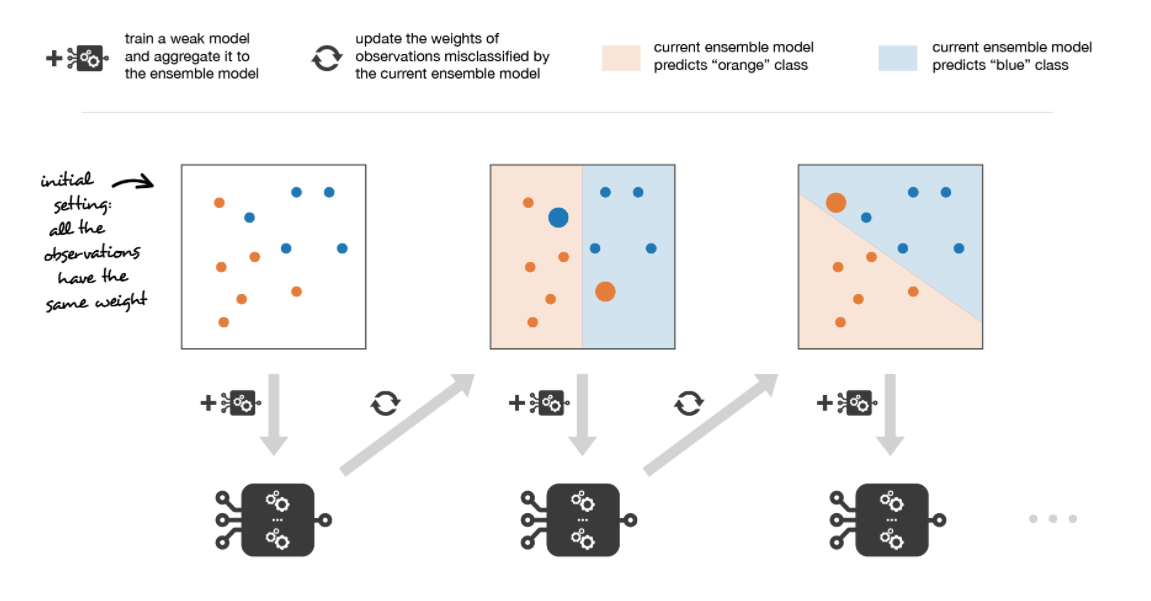
\includegraphics[scale=0.35]{ada.png}
		\caption{Esempio grafico dell'algoritmo AdaBoost.
		} 
		Source: \url{https://www.section.io/engineering-education/boosting-algorithms-python/}\label{fig:ada}
	\end{center}
\end{figure}
L'iperparametro da gestire in questo algoritmo è il numero di classificatori deboli da utilizzare, che verrà scelto attraverso la Cross Validation.\\
L'algoritmo AdaBoost risulta essere robusto contro l'\emph{overfitting}.
	
